\section{Performance Benchmarks of LoRAX Deployments}

To assess the viability of serving many LoRA fine-tuned LLMs simultaneously in a real-world application, we launch LoRA Land. LoRA Land is a web application that serves 25 fine-tuned Mistral-7b LLMs served to thousands of users from a single A100 GPU.

\begin{figure}[ht]
    \centering
    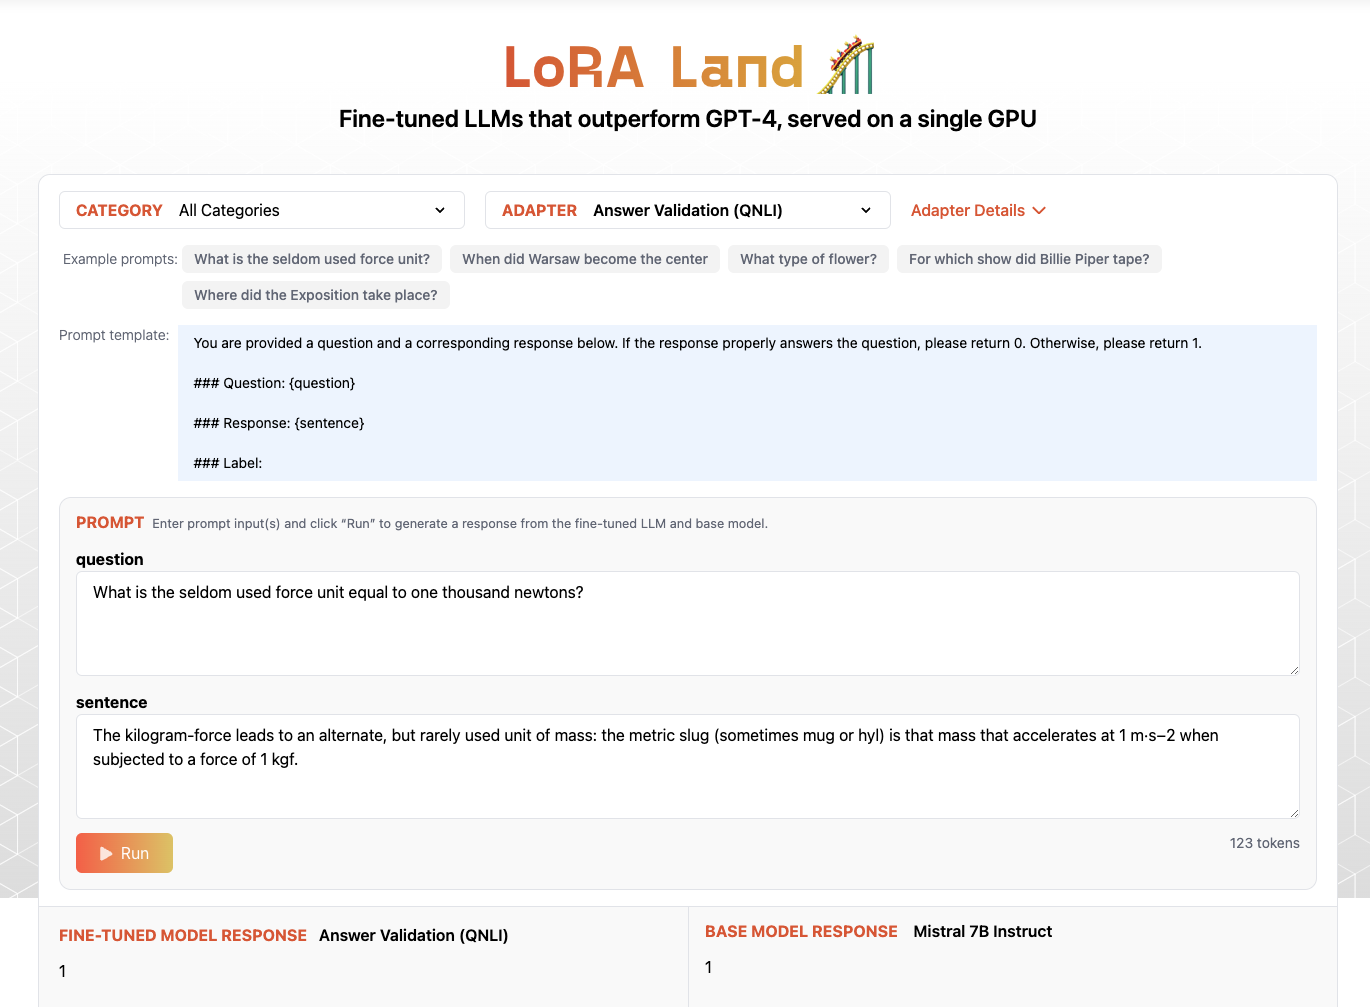
\includegraphics[width=\textwidth]{figures/lora_land.png}
    \vspace{5mm}
    \caption{The LoRA Land web application that serves 25 fine-tuned LLMs on a single A100. The application is available at \href{https://predibase.com/lora-land}{https://predibase.com/lora-land}.}
    \label{fig:loraland}
\end{figure}

\subsection{LoRAX in a Nutshell}

LoRA Exchange (LoRAX) \cite{12predibaseLoRAExchange} is an open source Multi-LoRA inference server specifically designed for serving many fine-tuned models at once using a shared set of GPU resources. Compared with conventional dedicated LLM deployments, LoRAX consists of three novel components:

\begin{itemize}
    \item \textbf{Dynamic Adapter Loading}, allowing each set of fine-tuned LoRA weights to be loaded from storage just-in-time as requests come in at runtime, without blocking concurrent requests.

    \item \textbf{Continuous Multi-Adapter Batching}, a fair scheduling policy for optimizing aggregate throughput of the system that extends the popular continuous batching strategy to work across multiple sets of LoRA adapters in parallel.

    \item \textbf{Tiered Weight Caching}, to support fast exchanging of LoRA adapters between requests, and offloading of adapter weights to CPU and disk to avoid out-of-memory errors.

\end{itemize}

\begin{figure}[ht]
    \centering
    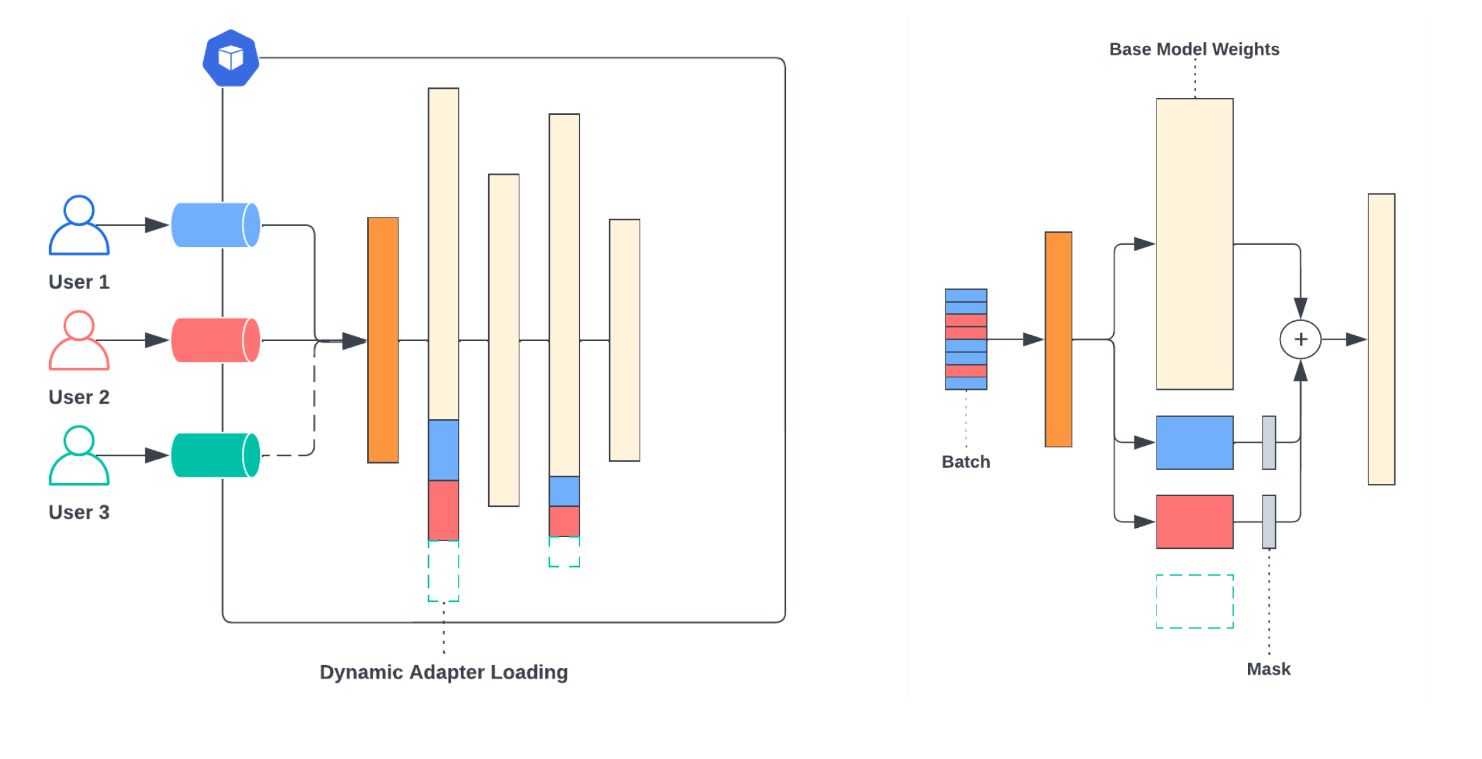
\includegraphics[width=\textwidth]{figures/lorax_nutshell.png}
    \caption{\textbf{Dynamic adapter loading} (left) enables multiple concurrent fine-tuned models to process requests. User 3’s model (green) is loaded in the background while the other requests proceed as usual. \textbf{Continuous Multi-Adapter Batching} (right): Multiple adapters are decoded in a single batch. Masks ensure that only the right adapter is used for processing each element of the batch.}
    \label{fig:loraxnutshell}
\end{figure}


\subsection{Benchmarking Results}

We run benchmarks in order to understand the impact of serving multiple adapters on the relevant metrics, described below. We also test the scalability of the system with respect to the following factors:

\begin{itemize}
\item Number of concurrent users submitting LLM prompts
\item Number of adapters concurrently being queried
\item Number of input tokens
\item Number of output tokens
\end{itemize}

LLM serving performance metrics include: time to first token (TFTT), total request time, token streaming time, and throughput (tokens per second). We run our benchmarks from a t3.2xlarge EC2 instance in the AWS zone us-west-2. All benchmarks are based on the Mistral-7b-instruct LLM, deployed on an A100 GPU with 80GB of RAM. The script used to benchmark LLM serving performance can be found in Appendix \ref{sec:appendixscripts}.

The following is a summary of relevant terminology:

\begin{itemize}

\item \textbf{Total request time (ms):} total time from when the request is sent to when the last token is streamed back to the client.
\item \textbf{Time to first token, TTFT (ms):} time from when the request is sent to the first token is received by the client
\item \textbf{Token streaming time (ms):} time from when the first token is received by the client to when the last token is received by the client.
\item \textbf{Throughput (token/s):} number of tokens generated per seconds, computed by (Token streaming time (ms) / number of output tokens)
\item \textbf{Concurrent users:} number of users that make requests to the LLM, wait until they receive a full response, then make another request until the end of testing time.

\end{itemize}

\subsection{Latency from adapter switching and concurrent users}

The following reported benchmarks come from 2-minute runs that continuously stream requests to the LLM deployment. Our experiments indicate that a duration of two minutes provides an adequate volume of data to obtain stable and reliable metrics.

Table \ref{table:adapterswitching} shows the impact LLM query performance isolated to adapter switching mechanics. In the multi-adapter, multi-user case, we see that the token streaming time is the same, but the total request time differs by 7.21ms which illustrates the cost of handling requests from 100 concurrent users that lead to switching between 25 adapters.

\begin{table*}[ht]
\centering

\scalebox{0.7}{
\begin{tabular}{rcccc}
\multicolumn{1}{c}{}           & \multicolumn{2}{c}{0 adapters (base model), 1 concurrent user} & \multicolumn{2}{c}{25 adapters (base model), 100 concurrent user} \\
\cmidrule(l{3pt}r{3pt}){2-3}\cmidrule(l{3pt}r{3pt}){4-5}
\multicolumn{1}{c}{}           & Average                        & p90                           & Average                          & p90                            \\
\midrule
Total request time (ms)        & 191.81                         & 192.3                         & 199.02                           & 201.82                         \\
Time to first token, TTFT (ms) & 122.19                         & 191.16                        & 128.79                           & 199.11                         \\
Token streaming time (ms)      & 70                             & 92.38                         & 70.14                            & 96.62                         
\end{tabular}
}

\caption{Measuring LLM querying metrics from adapter switching mechanics only. To eliminate extra, non-adapter-switching factors related to input and generation, simulated requests contain 1 input token and \textit{max\_new\_tokens} is capped at 1. Throughput metrics are excluded since only 1 output token is generated. \label{table:adapterswitching}}
\end{table*}


\begin{table}[ht]
\centering  
\footnotesize % Smaller font size to fit the table within the page width

\begin{tabular}{ccccccc}
\# concurrent users                             &         & 1       & 5       & 10      & 20      & 50      \\
\midrule
\multirow{2}{*}{Total request time (ms)}        & average & 943.03  & 1165.71 & 1359.39 & 2004.9  & 2981.66 \\
                                                & p90     & 1567.66 & 1925.96 & 2147.84 & 3287.21 & 4673.52 \\
\multirow{2}{*}{Time to first token, TTFT (ms)} & average & 121.84  & 121.80  & 143.68  & 135.43  & 136.17  \\
                                                & p90     & 191.08  & 195.85  & 199.98  & 199.76  & 199.54  \\
\multirow{2}{*}{Token streaming time (ms)}      & average & 821.09  & 1043.79 & 1215.6  & 1869.36 & 2845.38 \\
                                                & p90     & 1468.76 & 1804.16 & 2007.89 & 3130.72 & 4544.64
\end{tabular}
\vspace{5mm}
\caption{Benchmarking base LLM deployments on 1xA100 with queries that simulate real load.}
\end{table}

To simulate realistic traffic payloads, we generate random payloads with 30-500 input tokens and 1-120 output tokens, modeled off of the tasks defined in Table \ref{table:datasets}. We vary the number of concurrent users from 1 to 50, and payloads are issued randomly between 25 different adapter endpoints. 

When scaling from 1 to 50 concurrent users, which also increases load by 50X, the average time to first token (TTFT) is slightly affected (+21.84ms or 17.9\% increase). We see a 3.46X decrease in throughput for the same 50X increase in load.

\begin{table}[ht]

\scalebox{0.9}{
\begin{tabular}{lcccccc}
\# concurrent users                             & \multicolumn{1}{l}{} & 1       & 5       & 10      & 20      & 50      \\
\midrule
\multirow{2}{*}{Total request time (ms)}        & average              & 956.56  & 1272.16 & 1528.99 & 1896.1  & 3336.27 \\
                                                & p90                  & 1758.53 & 2164.08 & 2612.05 & 3222.73 & 5330.84 \\
\multirow{2}{*}{Time to first token, TTFT (ms)} & average              & 170.62  & 148.14  & 157.49  & 167.28  & 153.89  \\
                                                & p90                  & 199.36  & 198.98  & 199.41  & 200.99  & 200.2   \\
\multirow{2}{*}{Token streaming time (ms)}      & average              & 785.82  & 1123.91 & 1371.39 & 1728.71 & 3182.27 \\
                                                & p90                  & 1594.65 & 2023.33 & 2468.87 & 3047.92 & 5169.05
\end{tabular}
}

\vspace{5mm}
\caption{Benchmarking 25 adapters on 1xA100 with queries that simulate real load. \label{table:loraxconcurrentusers}}

\end{table}

Table \ref{table:loraxconcurrentusers} shows that there’s no significant difference between querying the base LLM vs. the 25 adapters when it comes to TTFT or throughput. The cost of adapter switching is overshadowed by the time it takes to generate tokens once requests come in. Comparing average case numbers vs. p90 numbers for TTFT, the largest disparity is between 121.8ms (average) and 195.95ms (p90) for a 60.87\% increase. Additionally, we consistently see that TTFT is at or under the 200ms mark.

On throughput, we observe that it takes between 12 and 13.5ms to generate a single token on an A100 GPU both for base deployments and deployments where adapter weights have been added. This means that the aggregate throughput for the LLM deployment on that GPU is between 74 tokens/s and 83 tokens/s.

\subsection{Analyzing the performance impact of additional deployment replicas}

In Table \ref{table:loraxreplicas}, we run benchmarks for 25 adapters queried concurrently by 50 users, with a LoRAX deployment on 1 replica. We then run benchmarks where we scale the LoRAX deployment to 2 replicas placed behind a round robin load balancer to route equal amounts of traffic to each replica, while also scaling the load to 100 concurrent users. We see that the numbers are stable across the board, signifying that replicas can be scaled linearly with load to achieve comparable metrics.


\begin{table}[ht]
\scalebox{0.8}{
\begin{tabular}{lccc}
                                                & \multicolumn{1}{l}{} & 50 Concurrent users, 1 replica & 100 Concurrent users, 2 replicas \\
\midrule
\multirow{2}{*}{Total request time (ms)}        & average              & 3336.27                        & 3368.53                          \\
                                                & p90                  & 5330.84                        & 5382.61                          \\
\multirow{2}{*}{Time to first token, TTFT (ms)} & average              & 153.89                         & 161.97                           \\
                                                & p90                  & 200.2                          & 199.83                           \\
\multirow{2}{*}{Token streaming time (ms)}      & average              & 3182.27                        & 3206.46                          \\
                                                & p90                  & 5169.05                        & 5248.97                         
\end{tabular}
}

\vspace{5mm}
\caption{Benchmarking 25 adapters on 1 LoRAX replica vs. 2 replicas with queries that simulate real load.}
\label{table:loraxreplicas}
\end{table}